\documentclass{article}

\usepackage[utf8]{inputenc}
\usepackage{amsthm}
\usepackage{amssymb}
\usepackage{mathtools}
\usepackage{graphicx}
\usepackage{mdframed}
\usepackage{float}
\usepackage[top=0.75in, bottom=0.75in, left=0.75in, right=0.75in]{geometry}
\usepackage{gauss}

\usepackage{array}
\allowdisplaybreaks

\makeatletter
\newcounter{elimination@steps}
\newcolumntype{R}[1]{>{\raggedleft\arraybackslash$}p{#1}<{$}}
\def\elimination@num@rights{}
\def\elimination@num@variables{}
\def\elimination@col@width{}
\newenvironment{elimination}[4][0]
{
    \setcounter{elimination@steps}{0}
    \def\elimination@num@rights{#1}
    \def\elimination@num@variables{#2}
    \def\elimination@col@width{#3}
    \renewcommand{\arraystretch}{#4}
    \start@align\@ne\st@rredtrue\m@ne
}
{
    \endalign
    \ignorespacesafterend
}
\newcommand{\step}[2]
{
    \ifnum\value{elimination@steps}>0\sim\quad\fi
    \left[
        \ifnum\elimination@num@rights>0
            \begin{array}
            {@{}*{\elimination@num@variables}{R{\elimination@col@width}}
            |@{}*{\elimination@num@rights}{R{\elimination@col@width}}}
        \else
            \begin{array}
            {@{}*{\elimination@num@variables}{R{\elimination@col@width}}}
        \fi
            #1
        \end{array}
    \right]
    & 
    \begin{array}{l}
        #2
    \end{array}
    \addtocounter{elimination@steps}{1}
}
\makeatother

\DeclarePairedDelimiter{\abs}{\lvert}{\rvert}
\DeclarePairedDelimiter{\norm}{\lvert \lvert}{\rvert \rvert}

\newtheoremstyle{break}% name
  {}%         Space above, empty = `usual value'
  {}%         Space below
  {\itshape}% Body font
  {}%         Indent amount (empty = no indent, \parindent = para indent)
  {\bfseries}% Thm head font
  {.}%        Punctuation after thm head
  {\newline}% Space after thm head: \newline = linebreak
  {}%         Thm head spec

\newtheorem{Def}{Definition}[section]

\theoremstyle{break}

\newtheorem{innerEx}{Exempel}[section]
\newtheorem{sats}{Sats}[section]
\newtheorem{Rem}{Anmärkning}[]

\newenvironment{Ex}
{\begin{mdframed} \begin{innerEx} \vspace{3pt}}
{\vspace{3pt} \end{innerEx} \end{mdframed}}  

\newenvironment{bevis}
{\begin{mdframed} \begin{proof} \vspace{3pt}}
{\vspace{3pt} \end{proof} \end{mdframed}}


\title{
	 Linjär Algebra\\
	 Föreläsning 12
    \author{Erik Sjöström}
}
\begin{document}
\maketitle

\section{Homogena ekvationssystem} % (fold)
\label{sec:homogena_ekvationssystem}
\begin{Ex}
    Låt $\mathbf{A} \cdot = \emptyset$ ges av:
    \[
        \begin{bmatrix} 
        3 & 0 & -1 & 0\\
        8 & 0 & 0 & -2\\
        0 & 2 & -2 & -1
        \end{bmatrix}
        \cdot
        \begin{bmatrix}
        x_1\\x_2\\x_3\\x_4
        \end{bmatrix}
        =
        \begin{bmatrix}
        0\\0\\0
        \end{bmatrix}
    \]
    En lösning är förstås:
    \[
        \begin{bmatrix} x_1\\x_2\\x_3\\x_4 \end{bmatrix} = 
        \begin{bmatrix} 0\\0\\0\\0 \end{bmatrix}
    \]
    Den lösningen kallas för den triviala lösning.\\
    Finns det fler lösningar? Vi gausseliminerar:
    \begin{elimination}[1]{4}{1.75em}{1.1}
    \step
    {
    3 & 0 & -1 & 0 & 0\\
    8 & 0 & 0 & -2 & 0\\
    0 & 2 & -2 & -1 & 0
    }
    {
    \\
    \cdot -\frac{8}{3}\\
    \\
    }
    \step
    {
    3 & 0 & -1 & 0 & 0\\
    0 & 0 & \frac{8}{3} & -2 & 0 \\
    0 & 2 & -2 & -1 & 0
    }
    {
    \\
    = R_3\\
    = R_2\\
    }
    \end{elimination}
    \begin{elimination}[1]{4}{1.75em}{1.1}
    \step
    {
    3 & 0 & -1 & 0 & 0\\
    0 & 2 & -2 & -1 & 0\\
    0 & 0 & \frac{8}{3} & -2 & 0
    }
    {
    \cdot \frac{1}{2}\\
    \cdot \frac{1}{2}\\
    \cdot \frac{1}{8/3}\\
    }
    \step
    {
    1 & 0 & -\frac{1}{3} & 0 & 0\\
    0 & 1 & -1 & -\frac{1}{2} & 0\\
    0 & 0 & 1 & -\frac{3}{4} & 0\\
    }
    {
    \\
    \\
    \\
    }
    \end{elimination}
    Låt $x_4 = t$, ($x_4$ är en fri variabel)\\
    Vi får:
    \[
        \begin{cases}
        	x_3 = \frac{3}{4} \cdot t\\
        	x_2 = \frac{3}{4} \cdot t + \frac{1}{2} \cdot t = \frac{5}{4} \cdot t\\
        	x_1 = \frac{1}{3} \cdot \frac{3}{4} \cdot t = \frac{1}{4} \cdot t
        \end{cases}
    \]
    Vi får alltså svaret:
    \[
        \begin{bmatrix} x_1\\x_2\\x_3\\x_4 \end{bmatrix} =
        \begin{bmatrix} 1/4\\5/4\\3/4\\1 \end{bmatrix} \cdot t
    \]
    Dvs: En linje i $\mathbb{R}^4$ genom origo.
\end{Ex}
\newpage
\noindent
Den homogena ekvationen $\mathbf{A} \cdot \vec{x} = \vec{b}$ har icke-trivial lösning omm reducering av totalmatrisen 
$\begin{bmatrix}
\begin{array}{c|c}
    \mathbf{A} & \emptyset
\end{array}
\end{bmatrix}$
till trappstegsform ger minst en fri kolumn.
\begin{sats}
    Antag att ekvationen $\mathbf{A} \cdot \vec{x} = \vec{b}$ har en lösning $\vec{x}_p$ (partikulärlösning). Då gäller att alla lösningar till $\mathbf{A} \cdot \vec{x} = \vec{b}$ kan skrivas som:
    \[
    \vec{x} = \vec{x}_p + \vec{x}_h
    \]
    Där $\vec{x}_h$ är lösningen till den homogena ekvationen:
    \[
    \mathbf{A} \cdot \vec{x} = \emptyset
    \]
\end{sats}
\begin{Ex}
    Vi ser på $\mathbf{A} \cdot \vec{x} = \vec{b}$ där:
    \begin{align*}
    & A = \begin{bmatrix} 1 & -2 & 1 \\ 0 & 2 & -8 \end{bmatrix}
    && \vec{b} = \begin{bmatrix} 0 \\ 8 \end{bmatrix}
    \end{align*}
    Radreducering ger:
    \begin{elimination}[1]{3}{1.75em}{1.1}
    \step
    {   
    1 & -2 & 1 & 0 \\
    0 & 2 & -8 & 8 \\
    }
    {
    + R_2\\
    \\
    }
    \step
    {
    1 & 0 & -7 & 8\\
    0 & 2 & -8 & 8\\
    }
    {
    \\
    \cdot \frac{1}{2}\\
    }
    \step
    {
    1 & 0 & -7 & 0\\
    0 & 1 & -4 & 4\\
    }
    {
    \\
    \\
    }
    \end{elimination}
    $x_3$ är en fri variabel. Låt $x_3=t$, $t \in \mathbb{R}$. Vi får:
    \begin{align*}
    &\begin{cases}
        x_1 = 8 + 7t\\
        x_2 = 4 + 4t\\
        x_3 = t\\
    \end{cases}
    &&\mbox{dvs}
    && \vec{x} = \overbrace{\begin{bmatrix} 8\\4\\0 \end{bmatrix}}^{\vec{x}_p} + \overbrace{\begin{bmatrix} 7\\4\\1 \end{bmatrix} \cdot t}^{\vec{x}_h}
    \end{align*}
\end{Ex}
\paragraph{Obs:} % (fold)
\label{par:obs_}
Vi har:
\begin{gather*}
    \mathbf{A} \cdot \vec{x}_p = \begin{bmatrix} 1 & -2 & 1\\0 & 2 & -8 \end{bmatrix} \cdot \begin{bmatrix} 8\\4\\0 \end{bmatrix} = \begin{bmatrix} 0\\8 \end{bmatrix}\\
    \mathbf{A} \cdot \vec{x}_h = \begin{bmatrix} 1 & -2 & 1\\0 & 2 & -8 \end{bmatrix} \cdot \begin{bmatrix} 7\\4\\1 \end{bmatrix} \cdot t = \begin{bmatrix} 0\\0 \end{bmatrix} \cdot t = \begin{bmatrix} 0\\0 \end{bmatrix}
\end{gather*}
\paragraph{Gemoetrisk tolkning:} % (fold)
\label{par:gemoetrisk_tolkning_}
Två plan som skär:
\begin{center}
    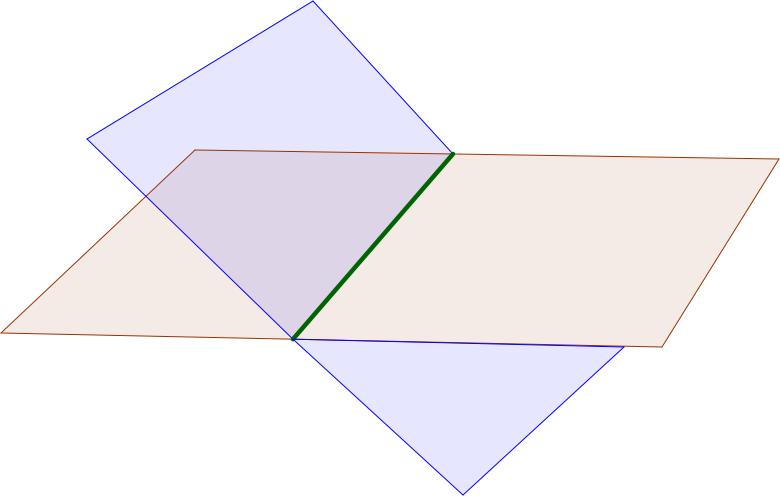
\includegraphics[scale=0.25]{tvaplan.png}
\end{center}
$\vec{x}_p  = \begin{bmatrix} 8\\4\\0 \end{bmatrix}$ är bara en av punkterna på linjen, nämligen den då $t=0$.\\
$\vec{x} = \vec{x}_p + \vec{x}_h$ är linjen i $\mathbb{R}^3$ förskjuten $\begin{bmatrix} 8\\4\\0 \end{bmatrix}$ från origo.
% paragraph gemoetrisk_tolkning_ (end)
% paragraph obs_ (end)
% section homogena_ekvationssystem (end)
\section{Överbestämda Ekvationssystem} % (fold)
\label{sec:_verbest_mda_ekvationssystem}
\begin{Def}
    Ett överbestämt ekvationssystem:
    \begin{itemize}
    	\item Fler ekvationer än obekanta.
    	\item Typexempel: Man har en mängd (mät)data som ska anpassas till någon funktion.
    \end{itemize}
\end{Def}
\begin{Ex}
\[
    \begin{array}{c|c|c|c|c|c|l}
    	t & 1 & 2 & 3 & 4 & 5 & \mbox{tid}\\
    	\hline
    	t & 3 & 5 & 8 & 10 & 13 & \mbox{uppmätt data}
    \end{array}
\]
\begin{center}
	INFOGA FIGUR HÄR	
\end{center}
Mätdatan blir nästan en linje, så man vill anpassa en rät linje:
\[
    y = k \cdot t + m
\]
till mätdatan. Då vill man att:
\begin{align*}
&&\begin{cases}
	3 = k \cdot 1 + m\\
	5 = k \cdot 2 + m\\
	8 = k \cdot 3 + m\\
	10 = k \cdot 4 + m\\
	13 = k \cdot 5 + m\\
\end{cases}
&&\Leftrightarrow
&&\begin{bmatrix} 1 & 1\\2 & 1\\3&1\\4&1\\5&1 \end{bmatrix}
\begin{bmatrix} k\\m \end{bmatrix} = 
\begin{bmatrix} 3\\5\\8\\10\\13 \end{bmatrix}
\end{align*}
Vi har alltså 5 ekvationer och 2 obekanta.
\begin{itemize}
	\item Det finns ingen exakt lösning eftersom punkterna ligger exakt på en linje.
	\item Vi vill hitta en lösning som blir så bra som möjligt i minsta kvadratmetodens mening
\end{itemize}
\end{Ex}
Titta på $\mathbf{A} \cdot \vec{x} = \vec{b}$ där:
\[
    \begin{bmatrix} 1&-2\\-1&3\\2&5 \end{bmatrix} \cdot \begin{bmatrix} x_1\\x_2 \end{bmatrix} = \begin{bmatrix} b_1\\b_2\\b_3 \end{bmatrix}
\]
kan skrivas som en linjärkombination:
\[
    \begin{bmatrix} 1\\-1\\2 \end{bmatrix} \cdot x_1 + \begin{bmatrix} -2\\3\\5 \end{bmatrix} \cdot x_2 = \begin{bmatrix} b1\\b_2\\b_3 \end{bmatrix}
\]
\begin{Def}
    \underline{Kolumnrummet} till en matris \textbf{A} är mängden av alla linjärkombinationer av kolumnerna i \textbf{A}.
\end{Def}
\begin{itemize}
	\item För ekvationen $\mathbf{A} \cdot \vec{x} = \vec{b}$ gäller att den har en lösning bara om $\vec{b}$ kan skrivas som en linjärkombination av kolumnerna i \textbf{A}.
	\item Kolumnrummet utgör ett plan, t.ex. alla linjärkombinationer av:
\end{itemize}
\begin{align*}
&\begin{bmatrix} 1\\-1\\2 \end{bmatrix}
&&\begin{bmatrix} -2\\3\\5 \end{bmatrix}
\end{align*}
utgör ett plan i $\mathbb{R}^3$
\begin{center}
	INFOGA FIGUR HÄR
\end{center}
Om $\vec{b}$ inte ligger i planet så saknas lösning till:
\[
    \mathbf{A} \cdot \vec{x} = \vec{b}
\]
Grundidén för minsta kvadratmetoden är att projicera högerledsekvationen $\vec{b}$ ortogonalt på kolumnrummer för \textbf{A} och sedan lösa ekvationen:
\[
    \mathbf{A} \cdot \vec{x} = \vec{b}_{\pi}
\]
där $\vec{b}_{\pi}$ är ortogonala projektionen.\\
På så vis fås en lösning $\vec{x}_0$ där avståndet:
\[
    \norm{\overbrace{\mathbf{A} \cdot \vec{x}_0}^{b_{\pi}} - \vec{b}} \le \norm{\overbrace{\mathbf{A} \cdot \vec{x}}^\text{En punkt} - \vec{b}}
\]
Låt:
\[
    \vec{r} = \mathbf{A} \cdot \vec{x}_0 - \vec{b}
\]
$\vec{r}$ är ortogonal mot kolumnerna i \textbf{A}. Dvs:
\[
    \mathbf{A}^T \cdot \vec{r} = \emptyset
\]
Dvs:
\[
    \emptyset = \mathbf{A}^T \cdot \vec{r} = \mathbf{A}^T \cdot (\mathbf{A} \cdot \vec{x}_0 - \vec{b}) = \mathbf{A}^T \cdot \mathbf{A} \cdot \vec{x}_0 - \mathbf{A}^T \cdot \vec{b} \Leftrightarrow \mathbf{A}^T \cdot \mathbf{A} \cdot \vec{x} = \mathbf{A}^T \cdot \vec{b}
\]
Med andra ord: $\vec{x}_0$ är lösningen till:
\[
    \mathbf{A}^T \cdot \mathbf{A} \cdot \vec{x} = \mathbf{A}^T \cdot \vec{b}
\]
\begin{Rem}
    Detta kallas för normalekvationen.
\end{Rem}
\begin{mdframed}
\paragraph{Exempel 2.1. (forts)} % (fold)
\label{par:exempel_2_1_}
\[
    \mathbf{A} \cdot \mathbf{A}^T = 
    \begin{bmatrix}
    1 & 2 & 3 & 4 & 5\\
    1 & 1 & 1 & 1 & 1\\
    \end{bmatrix} \cdot
    \begin{bmatrix}
    1 & 1\\
    2 & 1\\
    3 & 1\\
    4 & 1\\
    5 & 1\\
    \end{bmatrix} = 
    \begin{bmatrix}
    55 & 15\\
    15 & 5\\
    \end{bmatrix}
\]
Vi får normalekvationerna:
\[
    \mathbf{A}^T \cdot \mathbf{A} \cdot \vec{x} = \mathbf{A}^T \cdot \vec{b} = \begin{bmatrix} 55&15\\15&5 \end{bmatrix} \cdot \begin{bmatrix} k\\m \end{bmatrix} = \begin{bmatrix} 142\\39 \end{bmatrix}
\]
Med lösningen:
\[
    \begin{cases}
    	k = \frac{5}{2}\\
    	m = \frac{3}{10}\\
    \end{cases}
\]
Dvs vi får linjen:
\[
    y = k \cdot t + m = \frac{5}{2} \cdot t + \frac{3}{10}
\]
% paragraph exempel_2_1_ (end)
\end{mdframed}
% section _verbest_mda_ekvationssystem (end)
\end{document}